\chapter{Implementation}
In order to achieve the project objective, it was necessary to apprehend a clear and unified understanding of what software components were needed. The following paragraph and figure explain the current implementation of some key flows within the program.
\begin{figure}[H]
    \centering
    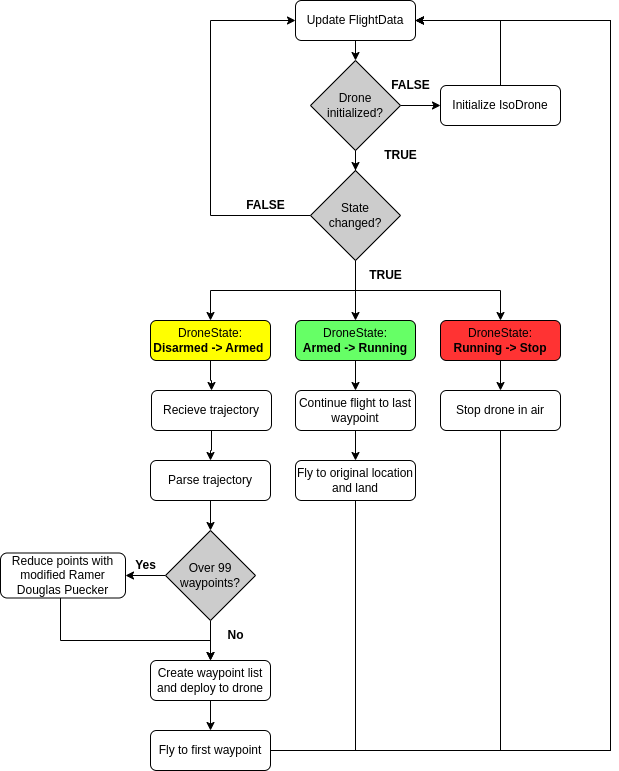
\includegraphics[scale=0.5]{figure/Flowchart-drone.png}
    \caption{Flowchart of parts of the drone program}
    \label{fig:drone-flow}
\end{figure}
The object-control module within the ATOS software facilitates the transmission of trajectories for drones and test objects in the local coordinate system, situated on the AstaZero test track through the ISO22133 protocol. The drone application subsequently receives this data when the state changes from Disarmed to Armed and turns the trajectory into global latitude and longitude coordinates through different functions. The application then transmits the trajectories to the drone by means of the DJI protocol, effectively initializing it. Following this, the test commences when the state is changed to "Running" in ATOS, and the drone and other test objects follow their pre-determined trajectories. Figure \ref{fig:drone-flow} displays this flow.


\section{Re-usability of existing software}
The AstaZero team has been developing an Android application for some time that the team could utilize. The code was open source and the team decided to contribute to the existing platform instead of creating a new one. This meant that some code functions vital to the project's success already existed.

\subsection{Iso-drone}
To establish a connection with the drone, the file IsoDrone provides a Java class that can be initiated to create a drone object able to communicate over the ISO22133 protocol. This meant that the team did not have to worry about the conversion of data into ISO-formatted strings but instead only could change variables of the current speed, heading, coordinates and similar and the drone object automatically transmitted this over the ISO22133 protocol. 
\\ \\
The protocol also enables the drone object to know what state ATOS is currently in and the application can set up triggers for when the state changes.

\subsection{Waypoint 1 Activity}
Since ATOS works with a local coordinate system, the location coordinates had to be converted to latitude and longitude coordinates in the Android application. This conversion was already present in the Waypoint1Activity file and works by bla bla bla \todo{Skriv hur den funkar med ett simpelt kodexempel} 

\subsection{Douglas-Peucker Algorithm}
With the WaypointMission limitations presented in section \ref{sec:limit_WP}, the AstaZero team made use of the Ramer-Douglas-Peucker algorithm, the algorithm is used for reducing the number of points in a curve while preserving its shape. %\todo{REFERERA!!!! http://www2.ipcku.kansai-u.ac.jp/~yasumuro/M_InfoMedia/paper/Douglas73.pdf}
This implementation made it possible to use trajectory files that normally would be composed of too many points to be run by the DJI waypointmission software. \\  

The algorithm divides the line recursively, starting with all points between the first and last one. The first and last points are automatically selected and retained, it then identifies the point that is the maximum distance from the line segment. If the point is more than a predefined tolerance away from the line segment, it must be selected as a new start- and endpoint, otherwise the point can be discarded without impacting the shape of the curve. The algorithm recursively calls itself on the two newly created segments and the process is repeated for each new line segment until all the points are outside of the given tolerance. The result is a new curve with fewer points that still closely approximates the original one. \\ 

This algorithm is heavily used when deploying curved trajectories to ISO-objects, especially drones but it also presents a problem when deploying trajectories that only consist of points in a straight line, it reduces too many points. The solution for this problem is presented in section \ref{sec:alt_douglas_peucker_algo} later in the chapter. 


\section{Implementation of drone trajectory}
\todo{Hitta nytt namn}

\section{Addition to Douglas-Puecker algorithm}
\label{sec:alt_douglas_peucker_algo}

The vast majority of the Douglas-Puecker implementation produced by the AstaZero team was used with only minor modification and additions. The problematic aspect of the algorithm was that it reduced too many points when presented with a trajectory in a straight line, leaving too few to points in the trajectory object to be sent to the next part of the point reduction implementation. The solution to this problem was to develop a simple collinearity check of the trajectory before applying the algorithm. If all points in the trajecotrie lies on a straight line 


\section{Implementation of image recognition}
\todo{Hitta nytt namn}

\section{Implementation of object tracking}
\todo{Hitta nytt namn}

\section{Integration and configuration}





% \subsection{Merging the apps}
% When both apps worked decently we tried merging the apps. Pretty quickly we realized the DJI SDK did not support running parallel missions in our case the waypoint mission and the activetrack mission. We are currently working on fixing this, by using the waypoint mission and running a convolutional neural network to identify cars on images from the video feed then using the pixel-coordinates of the object to adjust the gimbal.

